\documentclass[12pt, a4paper]{article}

\usepackage[utf8]{inputenc}
\usepackage[english]{babel}

\usepackage[margin=2cm]{geometry}

\usepackage[allowlitunits]{siunitx}

\usepackage{fontspec}
\usepackage{sectsty}

\setromanfont{Cambria}
\setmonofont[Scale=MatchLowercase]{Inconsolata}

\sectionfont{\bfseries\upshape\Large}
\subsectionfont{\bfseries\upshape\large}
\subsubsectionfont{\mdseries\upshape\normalsize}

\usepackage{hyperref}

\usepackage{graphicx}
\usepackage{float}

\usepackage{microtype}

\usepackage{booktabs}
\usepackage{array}

\usepackage{enumitem}

\usepackage{listings}
\lstset{basicstyle=\ttfamily}

\setlength{\parindent}{0em}
\setlength{\parskip}{0.5ex}

%\setcounter{tocdepth}{1}

\usepackage[sorting=none]{biblatex}

\addbibresource{references.bib}

\begin{document}

\begin{flushright}
\bfseries\upshape\Large
Data acquisition system for the RPC detector

Development documentation

by Pavel Demin
\end{flushright}

\tableofcontents

\section{Hardware}

An overview of the RPC detector with its data acquisition system is shown in figure \ref{fig:overview}.

\begin{figure}[h!]
  \centering
  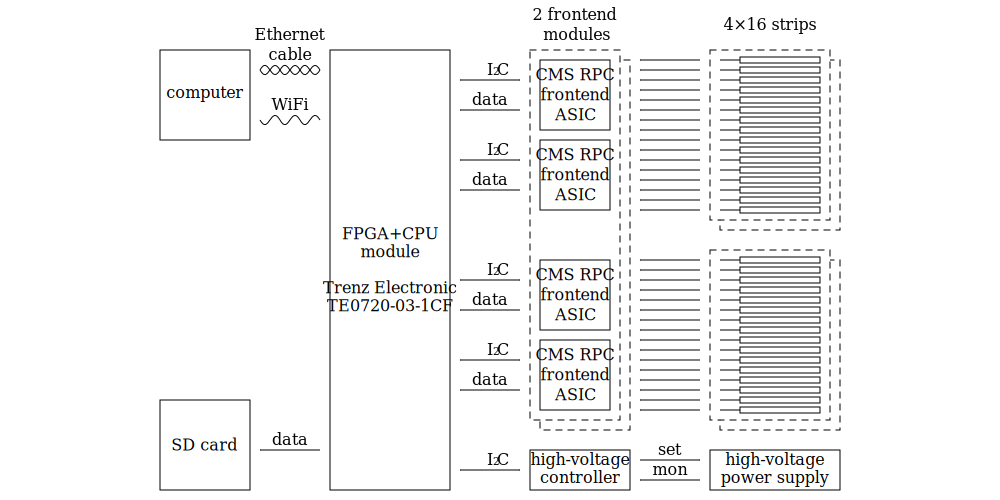
\includegraphics[width=\textwidth]{images/overview.pdf}
  \caption{overview of the RPC detector with its data acquisition system}
  \label{fig:overview}
\end{figure}

The data acquisition system consists of the following subsystems:
\begin{itemize}[nosep]
  \item 1 computer
  \item 1 FPGA+CPU module (Trenz Electronic TE0720-03-1CF) \cite{te0720}
  \item 1 high-voltage power supply (iseg DPS mini DPn 100 504 24 5 M) \cite{dpsmini}
  \item 1 high-voltage controller
  \item 2 frontend modules \cite{rpcfesch}
  \item 4 groups of 16 RPC strips connected to CMS RPC frontend integrated circuits \cite{rpcnim2000} in the frontend modules
\end{itemize}

\subsection{High-voltage controller}

The structure of the high-voltage controller is shown in figure \ref{fig:hvctrl_module}.

\begin{figure}[h!]
  \centering
  
\includegraphics[width=\textwidth]{images/hvctrl_module.pdf}
  \caption{structure of the high-voltage controller}
  \label{fig:hvctrl_module}
\end{figure}

The high-voltage controller can control up to four high-voltage power supplies and consists of the following components:
\begin{itemize}[nosep]
  \item 1 I/O expander for $\text{I}^\text{2}\text{C}$ bus (NXP PCF8574T) \cite{pcf8574t}
  \item 2 digital to analog and analog to digital converters (Analog Devices AD5593R) \cite{ad5593r}
\end{itemize}

The I/O expander for $\text{I}^\text{2}\text{C}$ bus is used to enable or disable individually each of the four high-voltage power supplies.

The DAC and ADC integrated circuits are used for controlling and monitoring the output voltage and current of the high-voltage power supplies.

\subsection{Frontend module}

The structure of the frontend module is shown in figure \ref{fig:rpcfe_module}.

\begin{figure}[h!]
  \centering
  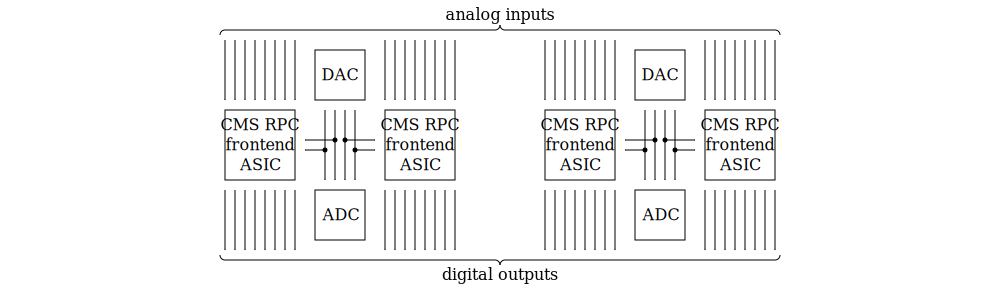
\includegraphics[width=\textwidth]{images/rpcfe_module.pdf}
  \caption{structure of the frontend module}
  \label{fig:rpcfe_module}
\end{figure}

The schematics of the frontend module can be found in \cite{rpcfesch}.

Each frontend module consists of the following components:
\begin{itemize}[nosep]
  \item 4 CMS RPC frontend integrated circuits \cite{rpcnim2000}
  \item 2 digital to analog converters (Analog Devices AD5316) \cite{ad5316}
  \item 2 analog to digital converters (Analog Devices AD7417) \cite{ad7417}
  \item 1 I/O expander for $\text{I}^\text{2}\text{C}$ bus (NXP PCF8574AT) \cite{pcf8574t}
\end{itemize}

The CMS RPC frontend integrated circuit has all the components necessary for conditioning and digitization of the analog signals coming from 8 RPC strips.

The DAC and ADC integrated circuits are used for controlling and monitoring the parameters of the CMS RPC frontend integrated circuits.

The I/O expander for $\text{I}^\text{2}\text{C}$ bus is used to enable or disable the DAC integrated circuits and to change their $\text{I}^\text{2}\text{C}$ addresses.

\subsection{CMS RPC frontend integrated circuit}

The structure of the CMS RPC frontend integrated circuit is shown in figure \ref{fig:rpcfe_ic}.

\begin{figure}[h!]
  \centering
  
\includegraphics[width=\textwidth]{images/rpcfe_ic.pdf}
  \caption{structure of the CMS RPC frontend integrated circuit}
  \label{fig:rpcfe_ic}
\end{figure}

The detailed information about the CMS RPC frontend integrated circuit can be found in \cite{rpcnim2000}, \cite{lhcb2002} and \cite{rpcreview2000}.

The 8 channels of the CMS RPC frontend integrated circuit operate independently. Each channel consists of a transimpedance preamplifier, a gain stage, a zero-crossing discriminator, a monostable multivibrator and a differential LVDS line driver.

The threshold of the zero-crossing discriminator and the duration of the output pulse of the monostable multivibrator are controlled by external voltage inputs $\text{V}_\text{threshold}$ and $\text{V}_\text{monostable}$. On the frontend module, these voltage inputs are connected to the outputs of the DAC integrated circuits.

\subsection{FPGA+CPU module}

The structure of the Trenz Electronic TE0720-03-1CF FPGA+CPU module is shown in figure \ref{fig:fpgacpu_module}.

\begin{figure}[h!]
  \centering
  
\includegraphics[width=\textwidth]{images/fpgacpu_module.pdf}
  \caption{structure of the FPGA+CPU module}
  \label{fig:fpgacpu_module}
\end{figure}

The Trenz Electronic TE0720-03-1CF FPGA+CPU module is based on the Xilinx Zynq XC7X020 system-on-chip (SOC) that integrates a dual-core ARM Cortex-A9 CPU and an FPGA on a single integrated circuit.

The FPGA is used to implement the time-to-digital converter (TDC) and the coincidence finding algorithm.

The module has 75 differential LVDS inputs/outputs to connect the FPGA to the 64 differential LVDS outputs of the frontend modules and to have additional inputs and outputs for test purposes.

The CPU with 1 GB of memory allows the Linux operating system and the data acquisition software to be run standalone.

The $\text{I}^\text{2}\text{C}$ interface is connected to all the integrated circuits (DAC, ADC and I/O expanders) that control the high-voltage power supply and the CMS RPC frontend integrated circuits on the frontend modules.

For connection to an external computer, it is possible to use the on-board Gigabit Ethernet interface or a WiFi module connected via the USB interface.

The SD card is used to record data during data acquisition runs and to store the Linux operating system, the FPGA configuration files and the data acquisition software.

\subsection{$\text{I}^\text{2}\text{C}$ bus}

All controllable integrated circuits on the high-voltage controller and on the frontend modules are connected to the same $\text{I}^\text{2}\text{C}$ bus which is controlled by the CPU on the FPGA+CPU module.

The addresses of the integrated circuits are shown in the following table:
\begin{center}
  \begin{tabular}{|l|l|}
  \hline
  \textbf{integrated circuit} & \textbf{address} \\
  \hline
  AD5593R on high-voltage controller & 0x10 \\
  \hline
  PCF8574T on high-voltage controller & 0x27 \\
  \hline
  AD7417 on frontend modules & 0x2A-0x2D \\
  \hline
  PCF8574AT on frontend modules & 0x38, 0x3C \\
  \hline
  AD5316 on frontend modules & 0x0E \\
  \hline
  \end{tabular}
\end{center}

\section{Software}

The software part of the data acquisition system consists of 15 subsystems represented by solid line blocks in figure \ref{fig:subsystems}.

\begin{figure}[h!]
  \centering
  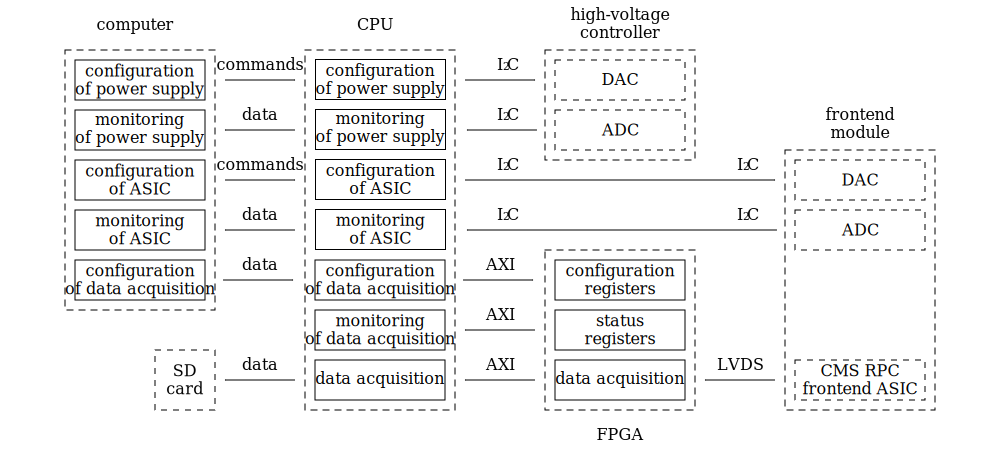
\includegraphics[width=\textwidth]{images/subsystems.pdf}
  \caption{software subsystems of the data acquisition system}
  \label{fig:subsystems}
\end{figure}

\subsection{Code organization}

The source code is stored in the GitHub repository at

\url{https://github.com/pavel-demin/giga-zee-notes}

This repository contains the following directories:
\begin{itemize}[nosep]
  \item \texttt{alpine} directory with the configuration files for Alpine Linux
  \item \texttt{cfg} directory with constraints and board definition files
  \item \texttt{cores} directory with IP cores written in Verilog
  \item \texttt{projects/muoscope} directory with the Vivado project written in Tcl
  \item \texttt{projects/muoscope/server} directory with the code of the data acquisition software
  \item \texttt{projects/muoscope/client} directory with the code of the graphical control and monitoring interface
  \item \texttt{scripts} directory with
  \begin{itemize}[nosep]
    \item Tcl scripts for Vivado and SDK
    \item shell script that builds the SD card image
  \end{itemize}
\end{itemize}

\subsection{Development environment}

The development machine must have the following software installed:
\begin{itemize}[nosep]
    \item Linux operating system (for example Debian 11 or Ubuntu 22.04)
    \item Xilinx toolchain (Vitis Core Development Kit 2020.2) \cite{vitis}
\end{itemize}

The packages required for the Xilinx toolchain and for the script that builds the SD card image can be installed with the following command:
\vspace{-1ex}
\begin{verbatim}
apt-get --no-install-recommends install \
  bc binfmt-support bison build-essential ca-certificates curl \
  debootstrap device-tree-compiler dosfstools flex fontconfig git \
  libgtk-3-0 libncurses-dev libssl-dev libtinfo5 parted qemu-user-static \
  squashfs-tools sudo u-boot-tools x11-utils xvfb zerofree zip
\end{verbatim}

\subsection{SD card image}

The SD card image is based on the lightweight Alpine Linux distribution \cite{alpine}.

The SD card image zip file with all necessary files can be built with the following commands:
\vspace{-1ex}
\begin{verbatim}
# setup Vitis and Vivado environment
source /opt/Xilinx/Vitis/2020.2/settings64.sh

# clone source code repository
git clone https://github.com/pavel-demin/giga-zee-notes

# go to giga-zee-notes directory
cd giga-zee-notes

# build SD card image zip file
source helpers/build-all.sh
\end{verbatim}

To prepare an SD card, simply unzip the SD card image zip file to an SD card with a single partition and a FAT32 file system.

\subsection{FPGA configuration}

The basic blocks of the FPGA configuration are shown in figure \ref{fig:fpga_configuration}.

\begin{figure}[h!]
  \centering
  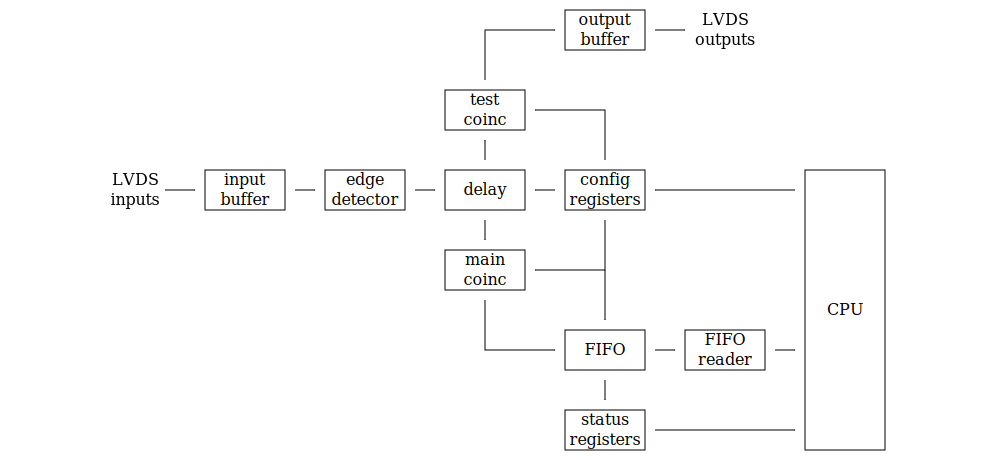
\includegraphics[width=\textwidth]{images/fpga_configuration.pdf}
  \caption{basic blocks of the FPGA configuration}
  \label{fig:fpga_configuration}
\end{figure}

The FGPA configuration contains the following addressable status and configuration registers:
\begin{center}
  \begin{tabular}{|l|l|}
  \hline
  \textbf{address} & \textbf{information} \\
  \hline
  0x40000000 + 0 & FIFO read counter (12-bit integer value) \\
  \hline
  0x40001000 + 0 & 3 reset bits (0: main coincidence reset, 1: test coincidence reset, 2: FIFO reset) \\
  \hline
  0x40001000 + 2 & delay configuration bits (0-3: RPC A, 4-7: RPC B, 8-11: RPC C, 12-15: RPC D) \\
  \hline
  0x40001000 + 4 & coincidence window (8-bit integer value) \\
  \hline
  0x40001000 + 5 & number of hit detectors (3-bit integer value) \\
  \hline
  \end{tabular}
\end{center}

Data in the FIFO buffer can be accessed by reading 32-bit values from address 0x40002000.

The FIFO read counter is used to check the presence of data in the FIFO buffer before reading it.

Reset bits are used to start and stop coincidence blocks and to empty the FIFO buffer.

Other configuration registers are used to configure the parameters of the delay and coincidence blocks.

The diagram of the coincidence finding algorithm is shown in figure \ref{fig:fsm}.

\begin{figure}[h!]
  \centering
  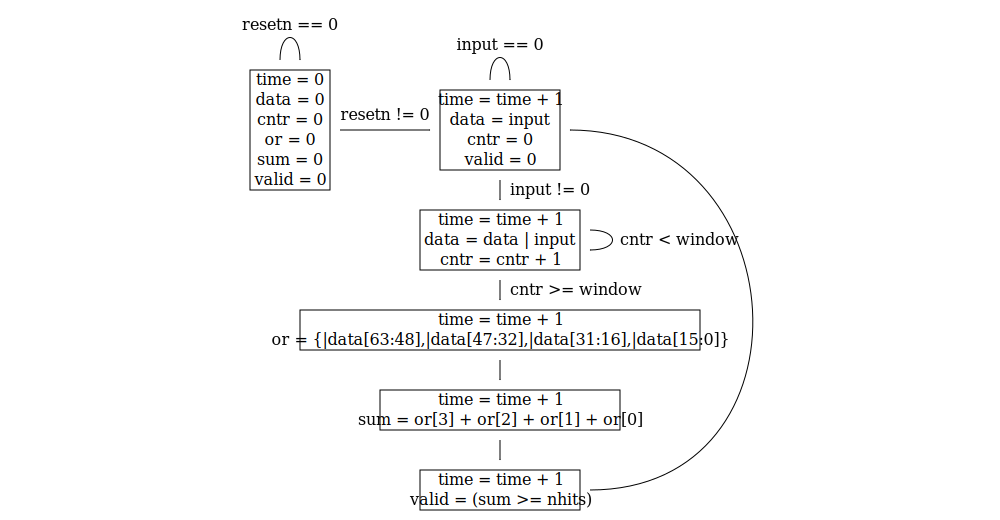
\includegraphics[width=\textwidth]{images/fsm.pdf}
  \caption{diagram of the coincidence finding algorithm}
  \label{fig:fsm}
\end{figure}

The FPGA clock frequency is set to 200 MHz and the time measurement accuracy is 5 ns.

The FPGA configuration can be built with the following commands:
\vspace{-1ex}
\begin{verbatim}
# setup Vitis and Vivado environment
source /opt/Xilinx/Vitis/2020.2/settings64.sh

# clone source code repository
git clone https://github.com/pavel-demin/giga-zee-notes

# go to giga-zee-notes directory
cd giga-zee-notes

# build muoscope.bit
make NAME=muoscope bit
\end{verbatim}

The FPGA can be configured from the command line of the FPGA+CPU module accessible via SSH:
\vspace{-1ex}
\begin{verbatim}
# send muoscope.bit to FPGA+CPU module using SCP
scp tmp/muoscope.bit root@192.168.42.1:apps/muoscope

# connect to FPGA+CPU module using SSH
ssh root@192.168.42.1

# go to apps/muoscope directory
cd apps/muoscope

# configure FPGA
cat muoscope.bit > /dev/xdevcfg
\end{verbatim}

\subsection{CPU configuration}

When the CPU boots, it loads and runs the secondary bootloader and the Linux operating system from the SD card. When ready, the Linux operating system configures all devices, including network interfaces and the FPGA, and starts all necessary services (DHCP, SSH, web interface, muoscope TCP server).

The WiFi interface is configured in hotspot mode with the network name (SSID) and password both set to \texttt{giga-zee}. The IP address of the WiFi interface is 192.168.42.1.

The Ethernet interface is configured to provide an IP address via DHCP to any directly connected computer. The IP address of the Ethernet interface is 192.168.43.1.

The default password for the \texttt{root} account is \texttt{changeme}.

\subsection{TCP server}

The \texttt{projects/muoscope/server/muoscope.c} file contains the source code of the TCP server that receives control commands and transmits the monitoring data to the graphical control and monitoring interface running on a remote computer.

The commands consist of 32 bits containing the following information:
\begin{center}
  \begin{tabular}{|l|r|}
  \hline
  \textbf{information} & \textbf{number of bits} \\
  \hline
  value & 16 \\
  \hline
  channel & 8 \\
  \hline
  code & 8 \\
  \hline
  \end{tabular}
\end{center}

When a command is received, the 8-bit code is used to identify the operation to be performed by the server:
\begin{center}
  \begin{tabular}{|c|l|}
  \hline
  \textbf{code} & \textbf{operation} \\
  \hline
  0 & read all ADC channels \\
  \hline
  1 & set DAC channel on the frontend modules \\
  \hline
  2 & set DAC channel on the high-voltage controller \\
  \hline
  3 & if value > 0 enable otherwise disable high-voltage power supply \\
  \hline
  4 & set delays \\
  \hline
  5 & set coincidence window \\
  \hline
  6 & set number of hit detectors \\
  \hline
  \end{tabular}
\end{center}

The C code of the TCP server can be compiled directly on the FPGA+CPU module with the following commands:
\vspace{-1ex}
\begin{verbatim}
# connect to FPGA+CPU module using SSH
ssh root@192.168.42.1

# go to apps/muoscope directory
cd apps/muoscope

# make SD card writable
rw

# compile
make

# make SD card read-only
ro
\end{verbatim}

\subsection{Graphical control and monitoring interface for interactive mode}

The graphical control and monitoring interface in the \texttt{projects/muoscope/client} directory is used to interactively control all subsystems during development and testing of the data acquisition system. This program runs on a computer that connects to the TCP server running on the FPGA+CPU module via the network using the TCP protocol.

The main window of the graphical control and monitoring interface is shown in figure \ref{fig:gui}.

\begin{figure}[h!]
  \centering
  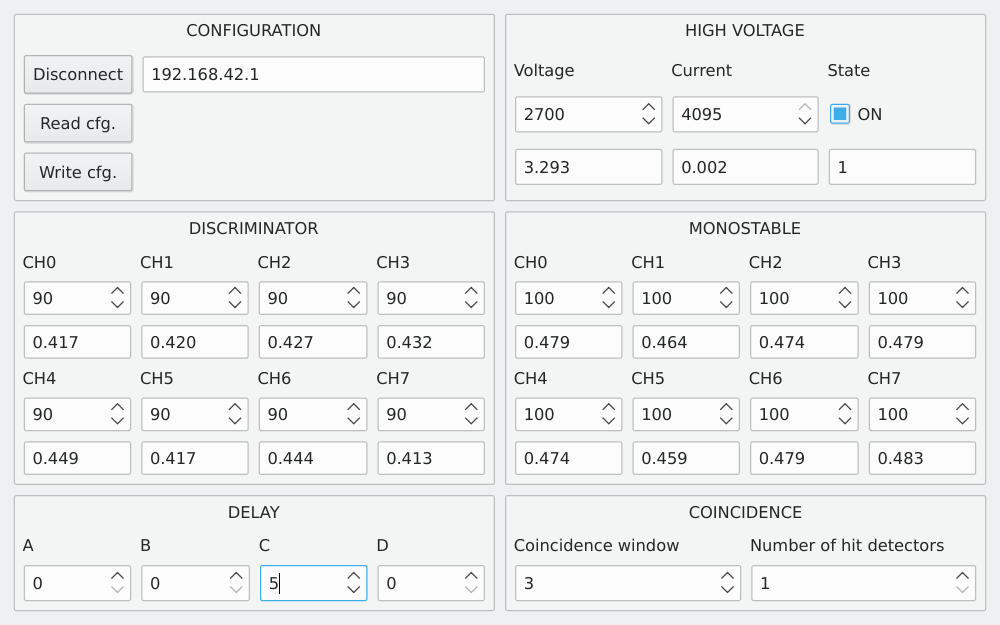
\includegraphics[width=0.8\textwidth]{images/gui.png}
  \caption{main window of the graphical control and monitoring interface}
  \label{fig:gui}
\end{figure}

The command to edit the layout of the main window is

\texttt{designer muoscope.ui}

The command to start the program is

\texttt{python3 muoscope.py}

After starting the program, it must be connected to the TCP server running on the FPGA+CPU module by entering the IP address (192.168.42.1 or 192.168.43.1) of the FPGA+CPU module in the input field in the upper left corner of the main window and pressing the "Connect" button.

The control elements are grouped together in five frames corresponding to each of the subsystems.

The control elements in the "HIGH VOLTAGE" frame are used to set the voltage, the current limit and to enable or disable the high-voltage power supply. The values in the input fields are expressed in units of the DAC part of the AD5593R integrated circuit on the high-voltage controller. The minimum value is 0 and the maximum value is 4095. Monitoring values are expressed in Volts as measured by the ADC part of the AD5593R integrated circuit on the high-voltage controller. The minimum value is 0V and the maximum value is 5V.

The control elements in the "DISCRIMINATOR" and "MONOSTABLE" frames are used to control $\text{V}_\text{threshold}$ and $\text{V}_\text{monostable}$ of each of the 8 CMS RPC frontend integrated circuits. The values in the input fields are expressed in units of the AD5316 DAC integrated circuits on the frontend modules. The minimum value is 0 and the maximum value is 1023. Monitoring values are expressed in Volts as measured by the AD7417 ADC integrated circuits on the frontend modules. The minimum value is 0V and the maximum value is 5V.

The input fields in the "DELAY" and "COINCIDENCE" frames are used to configure the parameters of the delay block and the coincidence algorithm in the FPGA. The values of the delays and coincidence window are expressed in number of FPGA clock cycles. The duration of the FPGA clock cycle is 5 ns.

\subsection{Command line interface for standalone data acquisition mode}

The \texttt{setup} and \texttt{dump} programs provide the command line interface for standalone data acquisition.

The \texttt{setup} program is used to set all the parameters of the high-voltage power supply and the CMS RPC frontend integrated circuits. When the \texttt{setup} program is run with no arguments, it prints the usage instructions:
\vspace{-1ex}
\begin{verbatim}
Usage: setup t0 t1 t2 t3 t4 t5 t6 t7 m0 m1 m2 m3 m4 m5 m6 m7 d0 d1 d2 d3 w n v c
 t0-t7 - threshold
 m0-m7 - monostable
 d0-d3 - delay
 w - window
 n - number of hit detectors
 v - voltage
 c - current
\end{verbatim}

After setting the parameters of the high-voltage power supply and the CMS RPC front-end integrated circuits, the data can be recorded to a file on the SD card using the \texttt{dump} program. When the \texttt{dump} program is run with no arguments, it prints the usage instructions:
\vspace{-1ex}
\begin{verbatim}
Usage: dump file
 file - output file
\end{verbatim}

When the \texttt{dump} program is running, it continuously reads data from the FIFO buffer in the FPGA and writes the data to a file on the SD card.

The data format is binary. Each record consists of 64 bits of hits data followed by 64 bits of timestamp. The bits corresponding to the channels having had a signal crossing the discriminator threshold during the coincidence window are set to 1. The timestamp is expressed in number of FPGA clock cycles. The duration of the FPGA clock cycle is 5 ns.

The following code is an example script using the \texttt{setup} program to set the voltage to values between 2000 and 3500 and the threshold to values between 80 and 100 and using the \texttt{dump} program to record data for 10 minutes for each combination of voltage and threshold values:
\vspace{-1ex}
\begin{verbatim}
for hv in `seq 2000 100 3500`
do
  for th in `seq 80 5 100`
  do
    file=scan_hv_${hv}_th_${th}.dat

    ./setup ${th} ${th} ${th} ${th} ${th} ${th} ${th} ${th} \
      100 100 100 100 100 100 100 100 0 0 0 0 4 1 ${hv} 4095

    sleep 10

    ./dump $file &

    sleep 600

    killall -q -s SIGINT dump
  done
done
\end{verbatim}

\newpage

\printbibliography

\end{document}